\begin{figure*}[h]
\centering
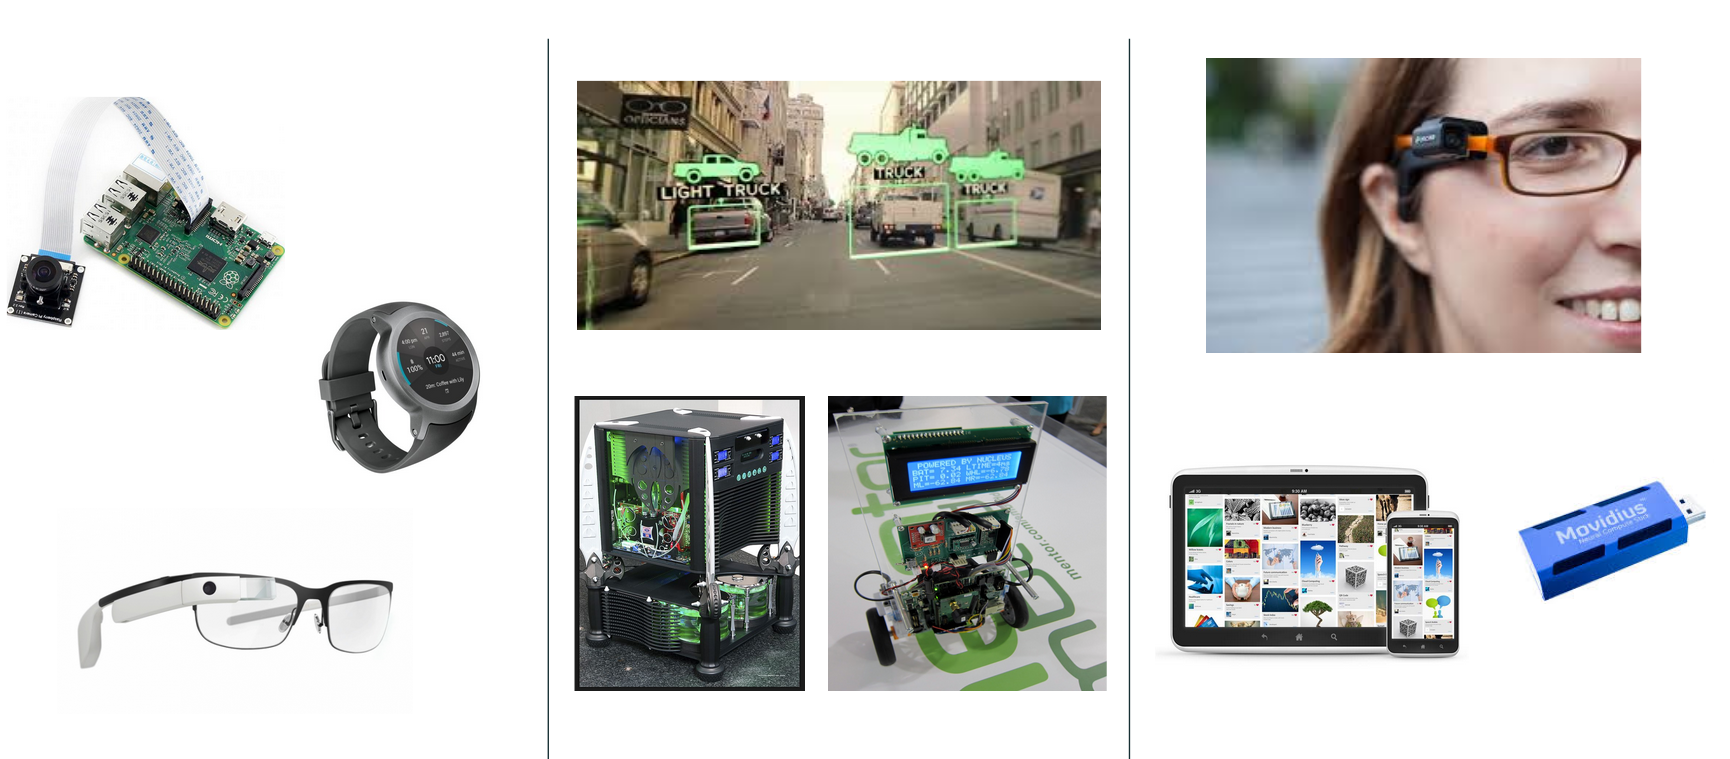
\includegraphics[width=0.9\textwidth]{figures/challenges.png}
\caption{There are two significant roadblocks to efficient deployment of large CNN models: realtime computation, and in-memory compactness. Cloud is not an option due to these real-time operation constraints.}
\label{fig:challenges}
%\vspace{-1.5cm}
\end{figure*}

\noindent Convolutional Neural Networks (CNNs) have found applications in many vision-related domains ranging from generic image-understanding for self-driving cars \cite{bojarski2016end} and automatic image captioning \cite{you2016image,johnson2016densecap} to recognition of specific image parts for scene-text recognition \cite{mishra2012top,neumann2012real} and face-based identification \cite{taigman2014deepface}. 

\noindent In the domain of image classification, AlexNet \cite{alex2012alexnet} and several architectural improvements  such as VGG-Net \cite{simonyan2014very} were proposed to push the limits of accuracy. These models were massive both in terms of memory usage and computational costs. AlexNet has around 60 million parameters in the network, while VGG has around 138 million, requiring 1.5 billion FLOPs and 19.6 billion FLOPs respectively for inference. The computational requirements make these architectures inappropriate for smaller portable systems such as mobiles and other embedded systems. These networks also consume large amounts of energy, creating a bottleneck for performance improvements. Full-precision multiply-accumulate (MAC) operations in floating point convolutional layers, for example, consumed 30x more power than integer MAC operations (see Table \ref{table:mac-energy}). These issues are addressed in two ways: (i) developing new compressed architectures (ii) compressing a given architecture.

\noindent There have been many developments in the area of model compression in the last few years, with the aim of bringing down runtimes and storage requirements to alleviate these challenges. Compression strategies for convolutional neural networks include architectural improvements \cite{he2016deep, iandola2016squeezenet}, reparametrization of fully connected layers \cite{moczulski2015acdc, yang2015deep}, pruning techniques \cite{han2015deep, liu2017learning}, and quantization \cite{courbariaux2016binarized, zhou2016dorefa}. Among these approaches, binarization and pruning  provided the most compact models as shown in Table \ref{table:versions_typesofcompression}. In this chapter, we motivate our exploration of binarization and pruning of convolutional neural networks, provide a background of methods explored in the past, and state the concrete contributions made in this thesis. 
 
\begin{table}[t]
\centering
\begin{tabular}{|l|c|}
\hline
{\bf Method} &  {\bf Compression} \\
\hline
Finetuned SVD 2 \cite{yang2015deep} & 2.6x \\
Circulant CNN 2 \cite{cheng2015exploration} & 3.6x \\
Adaptive Fastfood-16 \cite{yang2015deep} & 3.7x \\
Collins \etal \cite{collins2014memory} & 4x \\
Zhou \etal \cite{zhou2016less} & 4.3x \\
ACDC \cite{moczulski2015acdc} & 6.3x \\
Network Pruning \cite{han2015deep} & 9.1x \\
Deep Compression \cite{han2015deep} & 9.1x \\
GreBdec \cite{yu2017compressing} & 10.2x \\
Srinivas \etal \cite{srinivas2017training} & 10.3x \\
\hline
{\bf Guo \etal \cite{guo2016dynamic}} & {\bf 17.9x} \\
{\bf Binarization} & {\bf ${\approx}$32x} \\ 
\hline
\end{tabular}
\caption{Comparison of Binarization and other methods in terms of compression.}
\label{table:versions_typesofcompression}
\end{table}

\section{Quantization}

\noindent Quantized networks are networks where weights/activations are quantized into low-precision representations. These techniques achieve the best model compression and several promising directions have been explored in this domain  \cite{han2015deep}. They are classified into the categories based on the following questions:
\begin{enumerate}
\item How do they approximate the floating point values? 
\item Which part of the network do they quantize?
\end{enumerate}  

\noindent Weights are mainly appproximated by two broad methods: deterministic rounding and stochastic rounding. In deterministic rounding, there is an one-to-one mapping between the quantized value and the real value, while in stochastic quantization, there is a sampling distribution which assigns the quantized value. We constrain ourselves to deterministic rounding in this work, primarily due to it being implementable in hardware. There are two parts of a network which are targets of quantization: weights and activations. We take both steps, quantizing weights and activations to achieve compact models and lower computational cost.\\

\noindent Quantization has proven to be a powerful compression strategy, especially in its most extreme form: binarization. Binarization has enabled the use of XNOR-Popcount operations for vector dot products, which take much less time than full-precision Multiply-Accumulates (MACs), contributing to a huge speedup in convolutional layers \cite{rastegari2016xnor,courbariaux2016binarized} on a general-purpose CPU. Moreover, as each binary weight requires only a single bit to represent, one can achieve drastic reductions in run-time memory requirements. Previous research \cite{rastegari2016xnor,courbariaux2016binarized} shows that it is possible to perform weight and activation binarization on large networks with up to 58x speedups and approximately 32x compression ratios, albeit with significant drops in accuracy \cite{rastegari2016xnor}. Later works moved away from binary representations of weights/inputs to multi-bit representations. The reason for this was mainly the large accuracy drops observed in binary networks. \\
\begin{table}[t]
\begin{center}
\begin{tabular}{|l|c|c|c|c|}
\hline
{\bf Operation} & {\bf MUL} & {\bf Power} & {\bf ADD} & {\bf Power}\\ 
\hline
32-bit Float & 3.7pJ & 18.5x & 0.9pJ & 30x \\
16-bit Float & 1.1pJ & 5.5x & 0.4pJ &  13.3x\\
8-bit Integer & 0.2pJ & 1x & 0.03pJ & 1x \\
\hline
\end{tabular}
\end{center}
\caption{As shown by Horowitz \etal\cite{horowitz2014power}, power consumption for various operations at 45nm 0.9V. Observe that 8-bit integers require significantly less energy than their equivalent 32-bit floating point operations.}
\label{table:mac-energy}
\end{table}

 
\noindent  This leads to the natural question of whether, in theory, binary-representations of neural networks can be used at all to effectively approximate a full-precision network. If shown to be sufficient, the search for an accurate binarization technique is worthwhile, due to the large gains in speedups (due to binary operations rather than full-precision MACs) and compression compared to multi-bit representations. We also offer intuitions about how this technique might be effective in problems involving data that is binary in nature, such as sketches.\\ 
 
\noindent We then explore the problem of hybrid binarization of a network. We propose a technique devised from our investigation into the question as to {\it where and which quantities of a network should one binarize}, with respect to inputs to a layer -- to the best of our knowledge, this is the first work that explores this question. We observe that in a trained fully binarized model, binarization leads to minimal error in some layers and significant errors in others. Our proposed partition algorithm, when run on trained fully binarized models can design effective architectures. When these hybrid models are trained from scratch, they  achieve a balance between compression, speedup, energy-efficiency, and accuracy. We conduct extensive experiments applying our method to different model architectures on popular large-scale classification datasets over different domains. The resulting models achieve significant speedups and compression with significant accuracy improvements over a fully binarized network.

\section{Compact layers (Pruning)}

\noindent Network pruning is widely used technique for reducing the inference cost of deep  models  in  low-resource  settings.  A  typical  pruning  algorithm  is  a  three stage pipeline,  i.e.,  training  (a  large  model),  pruning  and  finetuning.   During  pruning, according to a certain criterion, redundant weights are pruned and important weights are kept to preserve the accuracy. All commonly used pruning techniques center around exploiting the sparsity in neural networks. A byproduct of pruning is that it removes redundancies during retraining, helping to prevent overfitting.\\

\noindent On the other hand, developing a compact layer for deep networks helps save memory and computational costs. Architectures such as ResNet \cite{he2016deep}, DenseNet \cite{huang2017densely} significantly reduced model size compared to VGG-Net by proposing a bottleneck structure to reduce the number of parameters while improving speed and accuracy. Additionally, they directed the focus of efficient designs of convolutional layers on increasing connectivity. Additional connectivity with residual connections to previous layers provided efficient information flow through the network, enabling them to achieve an order of magnitude reduction in storage and computational requirements. We take inspiration from these approaches, to focus on designing highly connected networks. We explore making networks efficient by designing sparse networks that preserve connectivity properties. \\

\noindent Recent architectures like MobileNet\cite{howard2017mobilenets} improves the efficiency by an order of magnitude over a ResNet. However, in order to achieve this, they sparsify a network by removing several connections from a trained network, reducing their accuracies in the process. We ask a basic question: If we try to maximize the connectivity properties and information flow, can we achieve the same efficiency gains with minimal loss in accuracy? It is essential that the connections allow information to flow through the network easily. That is, each output node must at least have the capacity to be sensitive to features of previous layers. Traditional model compression techniques such as pruning can aggravate the problem, since they can prune the neuron connections of a layer, while being agnostic of global connectivity of the network. A necessary condition for having good representational power is efficient information flow through the network, which is particularly suited to be modeled by graphs. \\

\noindent We propose to make the connections between neurons (filters in the case of CNNs) according to specific graph constructions known as expander graphs. They have been widely studied in spectral graph theory \cite{spielman2007spectral} and pseudorandomness \cite{salil2012pseudo}, and are known to be sparse but highly connected graphs. Expander graphs have a long history in theoretical computer science, also being used in practice in computer networks, constructing error correcting codes, and in cryptography (for a survey, see \cite{hoory2006expander}). 

\section{Contributions}

Overall, in this thesis we make the following contributions: 
\begin{enumerate}
\item Binarization
\begin{enumerate}
\item We show that binary representations are as expressive as full precision neural networks for polynomial functions, and offer theoretical insights into the same. 
\item We present a generalized, distribution-aware representation for binary networks, and proceed to calculate the generalized parameter-values for any binary network. We offer an intuitive analysis and comparison of our representation vis-a-vis existing representations.
\item We provide a provably efficient implementation of networks trained using this representation. We demonstrate the effectiveness of our method by extensive experiments applying it to popular model architectures on large-scale sketch datasets and improving upon existing binarization approaches.
\item We propose a metric to jointly optimize binarization-errors of layers and the associated computational costs and a partitioning algorithm to find suitable layers for input binarization, based on the above metric, which generates hybrid model architectures which if trained from scratch, achieve a good balance between compression, speedup, energy-efficiency, and accuracy.
\item Insights into what the algorithm predicts, which can provide an intuitive framework for understanding why binarizing certain areas of networks demonstrably achieves significant compression with respect to other compression methods; with hybrid model architectures for AlexNet, ResNet-18, Sketch-A-Net and SqueezeNet with over 5-8\% accuracy improvements on various datasets like Imagenet and TU-Berlin sketch recognition;
\end{enumerate}
\item Pruning (Compact Layer Design)
\begin{enumerate}
\item We propose to represent neuronal connections in deep networks using expander graphs (see Section \ref{sec:approach}). We further prove that X-Nets have strong connectivity properties (see Theorem \ref{thm:conn}).
\item We provide memory-efficient implementations of  Convolutional (X-Conv) layers using sparse matrices and propose a fast expander-specific algorithm and empirically compare X-Conv layers with grouped convolutions that have the same level of sparsity but worse connectivity. X-Conv layers obtain a 4\% improvement in accuracy when both the techniques are applied to the MobileNet architecture trained on Imagenet (see Section \ref{sec:group}).
\item We demonstrate the robustness of our approach by obtaining better performance trade-offs when applied to some of the state of the art models like DenseNet-BC and ResNet with a simple design, additionally achieving comparable compression rates to even the state-of-the-art trained pruning techniques.
\item Since we enforce the sparsity before the training phase itself, our models are inherently compact and faster to train compared to pruning techniques. We leverage this and showcase the performance of wider and deeper X-Nets. 
\end{enumerate}
\end{enumerate}

\noindent We shall be diving into the details of each contribution in chronological order in this thesis. The next chapter shall explore existing literature and pose our contributions in context and how the proposed contributions are novel.
